\documentclass{article}
\usepackage{qilin}
\tikzstyle{process} = [rectangle, rounded corners, minimum width=1.5cm, minimum height=0.5cm,align=center, draw=black, fill=gray!30, auto]
\title{AER372: Control Systems  \\ Assignment 1}
\author{QiLin Xue}
\date{Spring 2022}
\usepackage{mathrsfs}
\usetikzlibrary{arrows}
\usepackage{stmaryrd}
\usepackage{accents}
\newcommand{\ubar}[1]{\underaccent{\bar}{#1}}
\usepackage{pgfplots}
\numberwithin{equation}{section}
\usepackage{amsmath, amssymb, graphics, setspace}

\newcommand{\mathsym}[1]{{}}
\newcommand{\unicode}[1]{{}}

\newcounter{mathematicapage}
\begin{document}

\maketitle
\begin{enumerate}[label=\textbf{1.\arabic*}]
    \item The force balance on $M_1,M_2,M_3$ give, respectively,
    \begin{align}
        M_1\ddot{x}_1 &= u_1 + k_2(x_2-x_1) + k_1(-x_1) \\ 
        M_2\ddot{x}_2 &= u_2 + k_3(x_3-x_2) + k_2(x_1-x_2) \\ 
        M_3\ddot{x}_3 &= u_3 + k_3(x_2-x_3).
    \end{align}
    Note that the signs can be verified for each spring force term by checking that moving each mass to the right (and thus a positive $x_i$) would cause the force to have the correct sign.
    
    Note that we haven't accounted for damping effects. But damping effects have the same sign as the spring forces when $x_i,\dot{x}_i$ have the same sign.
    
    Therefore, In matrix form, this becomes:
    \begin{equation}
        \begin{pmatrix}
            M_1\ddot{x}_1 \\ 
            M_2\ddot{x}_2 \\ 
            M_3\ddot{x}_3
        \end{pmatrix} = \begin{pmatrix}
            -k_2-k_1 & k_2 & 0 \\ 
            k_2 & -k_2-k_3 & k_3 \\
            0 & k_3 & -k_3 
        \end{pmatrix}\begin{pmatrix}
            x_1 \\ x_2 \\ x_3
        \end{pmatrix} + \begin{pmatrix}
            -b_2-b_1 & b_2 & 0 \\ 
            b_2 & -b_2-b_3 & b_3 \\
            0 & b_3 & -b_3 
        \end{pmatrix}\begin{pmatrix}
            \dot{x}_1 \\ \dot{x}_2 \\ \dot{x}_3
        \end{pmatrix} + \begin{pmatrix}
            u_1(t) \\ 
            u_2(t) \\ 
            u_3(t)
        \end{pmatrix}.
    \end{equation}
    \item Assuming the wheels roll without slipping, the cart will instantaneously rotate about a fixed point. This fixed point can be constructed by drawing perpendicular lines from all the wheels and seeing where they intersect. Consider the below diagram,
    \begin{center}
        \begin{tikzpicture}
            % Draw a rectangle from (0,0) to (2,1)
            \draw[thick] (0,0) rectangle (6,2);

            % Draw the front wheel
            \draw[ultra thick] (4.8,0.6) -- (5.6,1.4);

            % Draw the two back wheels
            \draw[ultra thick] (0.6,1.4) -- (1.8,1.4);
            \draw[ultra thick] (0.6,0.6) -- (1.8,0.6);

            % Draw center of mass
            \draw[thick] (3,1) circle (0.1);

            % Draw a plus
            \draw[thick] (3,1.1) -- (3,0.9);
            \draw[thick] (2.9,1) -- (3.1,1);

            % Draw dotted lines perpendicular to the previous lines
            % They intersect at a pivot
            \draw[dotted] (1.2,0.6) -- (1.2, 5);
            \draw[dotted] (5.2, 1) -- (1.2, 5);

            % Draw angle between two dotted lines
            \draw[thick] (1.2, 4.5) arc (270:315:0.5);

            % Angle text
            \node at (1.5, 4.3) {$\theta_s$};

            % Draw line between pivot and center of mass
            \draw[dotted] (3,1) -- (1.2, 5);

            
            % Draw angle between two dotted lines
            \draw[thick] (1.2, 3.8) arc (270:295:1.2);

            % Angle text
            \node at (1.5, 3.6) {$\theta_s'$};

            % Draw velocity vector of front whel
            \draw[thick, blue, ->] (5.6,1.4) -- (6.6,2.4);
            % Label with V0
            \node[blue] at (6.8,2.4) {$V_0$};

            % Draw velocity vector of COM
            \draw[thick, red, ->] (3,1) -- (4.2,1.7);

            % Label with V_{CM}
            \node[red] at (4.3,1.4) {$V_\text{CM}$};

            % Label first dotted line with R
            \node at (3.5, 3.2) {$R$};

            % Label middle dotted line with R'
            \node at (2.5, 2.8) {$R'$};

            % Draw distance between wheels and COM with L/2
            % \draw[thick, <->] (3,-0.3) -- (5.2, -0.3) node[midway, below]{$L/2$};

            % Draw distance between back wheels and COM with L/2
            \draw[thick, <->] (1.2,-0.3) -- (5.2, -0.3) node[midway, below]{$L$};   

            % Draw an X between the two back wheels
            \draw[thick] (1.1,0.9) -- (1.3,1.1);
            \draw[thick] (1.1,1.1) -- (1.3,0.9);
        \end{tikzpicture}
    \end{center}
    We have:
    \begin{align}
        \sin\theta_s = \frac{L}{R},\quad\quad\quad\quad\quad \sin\theta_s' = \frac{L}{2R'}.
    \end{align}
    The angular frequency of every point on the robot is the same $\omega_n = \frac{V_0}{R}.$ Therefore,
    \begin{align}
        V_{CM} &= \omega_n R' \\ 
        &= \frac{V_0}{R} \frac{L}{2\sin\theta_s'} \\ 
        &= \frac{V\sin\theta_s}{2\sin\theta_s'}.
    \end{align}
    The naive idea here is to say the lateral velocity is $V_{CM}\sin\theta_s',$ but note that the robot could already be rotated. Let the angle of rotation with respect to the horizontal line be $\alpha,$ so we have:
    \begin{equation}
        V_{CM,lat} = V_{CM}\sin(\theta_s' + \alpha).
    \end{equation}
    Using the sine addition formula, we can simplify this to 
    \begin{align}
        V_{CM,lat} &= V_{CM}\sin\theta_s'\cos\alpha + V_{CM}\cos\theta_s'\sin\alpha \\
        &=\frac{V_0}{2}\sin\theta_s \cos\alpha + \frac{V_0\sin\theta_s}{2\tan\theta_s'}\sin\alpha.
    \end{align}
    To simplify this, note that we can write:
    \begin{align}
        \frac{\sin\theta_s}{\tan\theta_s'} = 2,
    \end{align}
    where we used the fact that 
    \begin{equation}
        \sin\theta_s \approx \tan\theta_s = 2\tan\theta_s' \approx 2\sin\theta_s'.
    \end{equation}
    Then,
    \begin{align}
        \dot{y}_{CM} &= \frac{V_0}{2}\theta_s + V_0\alpha.
        % \ddot{y} &= \frac{V_0}{2}\dot{\theta}_s + V_0\dot{\alpha} \\ 
        % &= \frac{V_0}{2}\dot{\theta}_s + \frac{2V_0}{L}\dot{y} \\ 
        % \dddot{y} &= \frac{V_0}{2}\ddot{\theta}_s + \frac{2V_0}{L}\ddot{y},
    \end{align}
    At the center of the two back wheels (marked with an X), the speed is 
    \begin{equation}
        V_{back} = R\cos\theta_s \omega_n = V_0\cos\theta_s \approx V_0
    \end{equation}
    so its lateral velocity is 
    \begin{equation}
        \dot{y}_{back} = V_0\sin\alpha \approx V_0\alpha.
    \end{equation}
    Note that the angle $\alpha$ can be written as 
    \begin{equation}
        \alpha \approx \sin\alpha = \frac{y_{CM}-y_{back}}{(L/2)}  \implies \dot{\alpha} = \frac{2}{L}\left({\dot{y}_{CM}-\dot{y}_{back}} \right) = \frac{V_0}{L}\theta_s.
    \end{equation}
    Taking higher derivatives of $\dot{y}_{CM},$ we have 
    \begin{align}
        \ddot{y}_{CM} &= \frac{V_0}{2}\dot{\theta}_s + V_0\dot{\alpha} \\
        &= \frac{V_0}{2}\dot{\theta}_s + \frac{V_0^2}{L}\theta_s.
    \end{align}
    Taking the derivative again, we have 
    \begin{equation}
        \dddot{y}_{CM} = \frac{V_0}{2}\ddot{\theta}_s + \frac{V_0^2}{L}\dot{\theta}_s.
    \end{equation}
    Recall that $U_{steer}=\dot{\theta}_s,$ so we have our final equation:
    \begin{equation}
        \boxed{\dddot{y}_{CM} = \frac{V_0}{2}\dot{U}_{steer} + \frac{V_0^2}{L}U_{steer}.}
    \end{equation}
    % where we used the fact that 
    % \begin{equation}
    %     \alpha \approx \tan\alpha = \frac{y}{L/2}
    % \end{equation}
    % is the angle the robot makes with the horizontal. Substituting in $\ddot{y},$ we arrive at 
    % \begin{align}
    %     \dddot{y} &= \frac{V_0}{2}\ddot{\theta}_s + \frac{2V_0}{L}\left(\frac{V_0}{2}\dot{\theta}_s + \frac{2V_0}{L}\dot{y}\right) \\ 
    %     &= \frac{V_0}{2}\ddot{\theta}_s + \frac{2V_0}{L}\left(\frac{V_0}{2}\dot{\theta}_s + \frac{2V_0}{L}\left(\frac{V_0}{2}\theta_s + V_0\alpha\right)\right) \\ 
    %     &= \frac{V_0}{2}\ddot{\theta}_s + \frac{V_0^2}{L}\dot{\theta}_s + \frac{2V_0^3}{L^2}\theta_s + \frac{4V_0^3}{L^2}\alpha \\ 
    %     &= \frac{V_0}{2}\ddot{\theta}_s + \frac{V_0^2}{L}\dot{\theta}_s + \frac{2V_0^3}{L^2}\theta_s + \frac{8V_0^3}{L^3}y. \\ 
    % \end{align} 
    % Assuming the wheels roll without slipping, the back two wheels will follow the first wheel, such that if the front of the robot (location of the center of the front wheel) moves a lateral distance of $d,$ the center of mass will move a lateral distance of $d/2.$ This is because the distance between the COM and the back wheels is equal to the distance between the COM of the front wheels, and this can be seen with simple geometry (i.e. similar triangles).
    
    % Let $y$ be the lateral distance. Then,
    % \begin{equation}
    %     \dot{y}_\text{front wheel} = V_0\sin\theta_s.
    % \end{equation}
    % But since the COM only moves half the distance, its speed is half, and thus 
    % \begin{equation}
    %     \dot{y}_{CM} = \frac{1}{2}V_0\sin\theta_s.
    % \end{equation}
    % The input is the rate of change of this angle, so we can write 
    % \begin{equation}
    %     \theta_s = \int_{0}^{t} U_\text{steer}\dd{t},
    % \end{equation}
    % to get our dynamic equation
    % \begin{equation}
    %     \boxed{\dot{y}_{CM} = \frac{1}{2}V_0\int_0^t U_\text{steer}\dd{t}},
    % \end{equation}
    % where we have further applied the $\sin \theta_s \approx \theta_s$ approximation since we are given that the angle is small.
    \item Let $I$ be the moment of inertia of the wheel, and let $\tau$ be the torque provided by the servo motor. A torque balance then gives,
    \begin{equation}
        I\ddot{\theta} = 2\tau - F_\text{fr,front}, 
    \end{equation}
    where $F_\text{fr,front}$ is the force of the static friction of the front wheel. Because the wheels are rolling without slipping, they must all be rotating at the same rate, and thus have the same angular acceleration. Torque balance on the other two wheels give 
    \begin{equation}
        I\ddot{\theta} = F_\text{fr,back}.
    \end{equation}
    Notice that $F_{fr,front},F_{fr,back}$ are all positive quantities when the robot is accelerating. For the front wheel, the supplied torque causes the wheel to turn while friction ensures it rotates without slipping and for the back wheels, it is the friction causing the wheel to turn. Newton's second law, substituting $a=R^2\ddot{\theta}$ for the condition of rolling without slipping, where $R$ is the radius of the wheel, we get 
    \begin{equation}
        MR^2\ddot{\theta} = F_{\text{fr,front}} - 2F_{\text{fr,back}},
    \end{equation}
    where $M$ is the mass of the robot. Substituting expressions for both friction, we arrive at 
    \begin{equation}
        MR^2\ddot{\theta} = 2\tau - 3I\ddot{\theta},
    \end{equation}
    or 
    \begin{equation}
        \ddot{\theta} = \frac{2\tau}{MR^2+3I}.
    \end{equation}
    The speed of the front wheel is given by,
    \begin{align}
        &V_0 = R\dot{\theta} \\ 
        \implies &\boxed{ \dot{V}_0 =\frac{2R\tau}{MR^2+3I}}
    \end{align}
    \item \begin{enumerate}[label=(\alph*)]
        \item Recall the power series
        \begin{equation}
            \cos t = 1 - \frac{1}{2!}t^2 + \frac{1}{4!}t^4 - \cdots = \sum_{n=0}^{\infty} \frac{(-1)^n}{(2n)!}t^{2n}.
        \end{equation}
        Then,
        \begin{align}
            \mathcal{L}\{g(t)\}(s) &= \sum_{n=0}^{\infty} \frac{(-1)^n}{(2n)!} \mathcal{L}\{t^{2n}f(t)\}(s) \\ 
            &= \sum_{n=0}^{\infty} \frac{(-1)^n}{(2n)!} (-1)^{2n} F^{(2n)}(s) \\ 
            &= \sum_{n=0}^{\infty} \frac{(-1)^n F^{(2n)}(s)}{(2n)!}.
        \end{align}
        Equivalently, this is the \textit{even} part of the function $F(s),$ with the added condition where the sign of each $x^{4i+2}$ term is flipped. This is:
        \begin{equation}
           \boxed{ \frac{1}{2}\left(F(js)+F(-js)\right)}
        \end{equation}
        \item Consider first the substitution $h(t_1):=\int_{0}^{t_1}f(\tau)\dd{\tau},$ where $h(t)$ has a Laplace transform of $H(s).$ Then,
        \begin{align}
            \mathcal{L}\{g(t)\}(s) &= \mathcal{L}\left\{\int_0^t h(t_1)\dd{t}_1\right\}(s) \\ 
            &= \frac{1}{s}H(s).
        \end{align}
        Similarly,
        \begin{align}
            H(s) &= \mathcal{L}\left\{\int_0^t f(\tau)\dd{\tau}\right\}(s) \\ 
            &= \frac{1}{s}F(s).
        \end{align}
        Therefore, the Laplace transform is 
        \begin{equation}
            \boxed{\frac{1}{s^2}F(s)}.
        \end{equation}
    \end{enumerate}
    \item The response to the unit step function $u(t)$ is given by
    \begin{equation}
        y(t) = \int_{-\infty}^{\infty} u(t)h(t-\tau) \dd{\tau} = u(t) * h(t).
    \end{equation}
    Note that we can rewrite 
    \begin{equation}
        h(t) = u(t) -u(t-2).
    \end{equation}
    Therefore,
    \begin{align}
        y(t) &= (u(t)-u(t-2)) * u(t) \\ 
        &= u(t)*u(t) - u(t-2)*u(t) \\ 
        &= R(t) - R(t-2),
    \end{align}
    where 
    \begin{equation}
        R(t) = \begin{cases}
            t & t\ge 0 \\ 
            0 & \text{else}
        \end{cases}
    \end{equation}
    is the ramp function. In the above computation, we applied linearity and the shifting function of convolutions.
    \item Let's first simplify the inner part of the diagram, which appears to be composed of two feedback loops juxtaposed on each other. We will show that the two leftmost summing points can be combined into a single summing point.
    
    Let the input be $R_1(s),$ and the output of the two summing points be $R_2(s)$ and $R_3(s),$ as shown in part (A) of the diagram below. 
    \begin{center}
        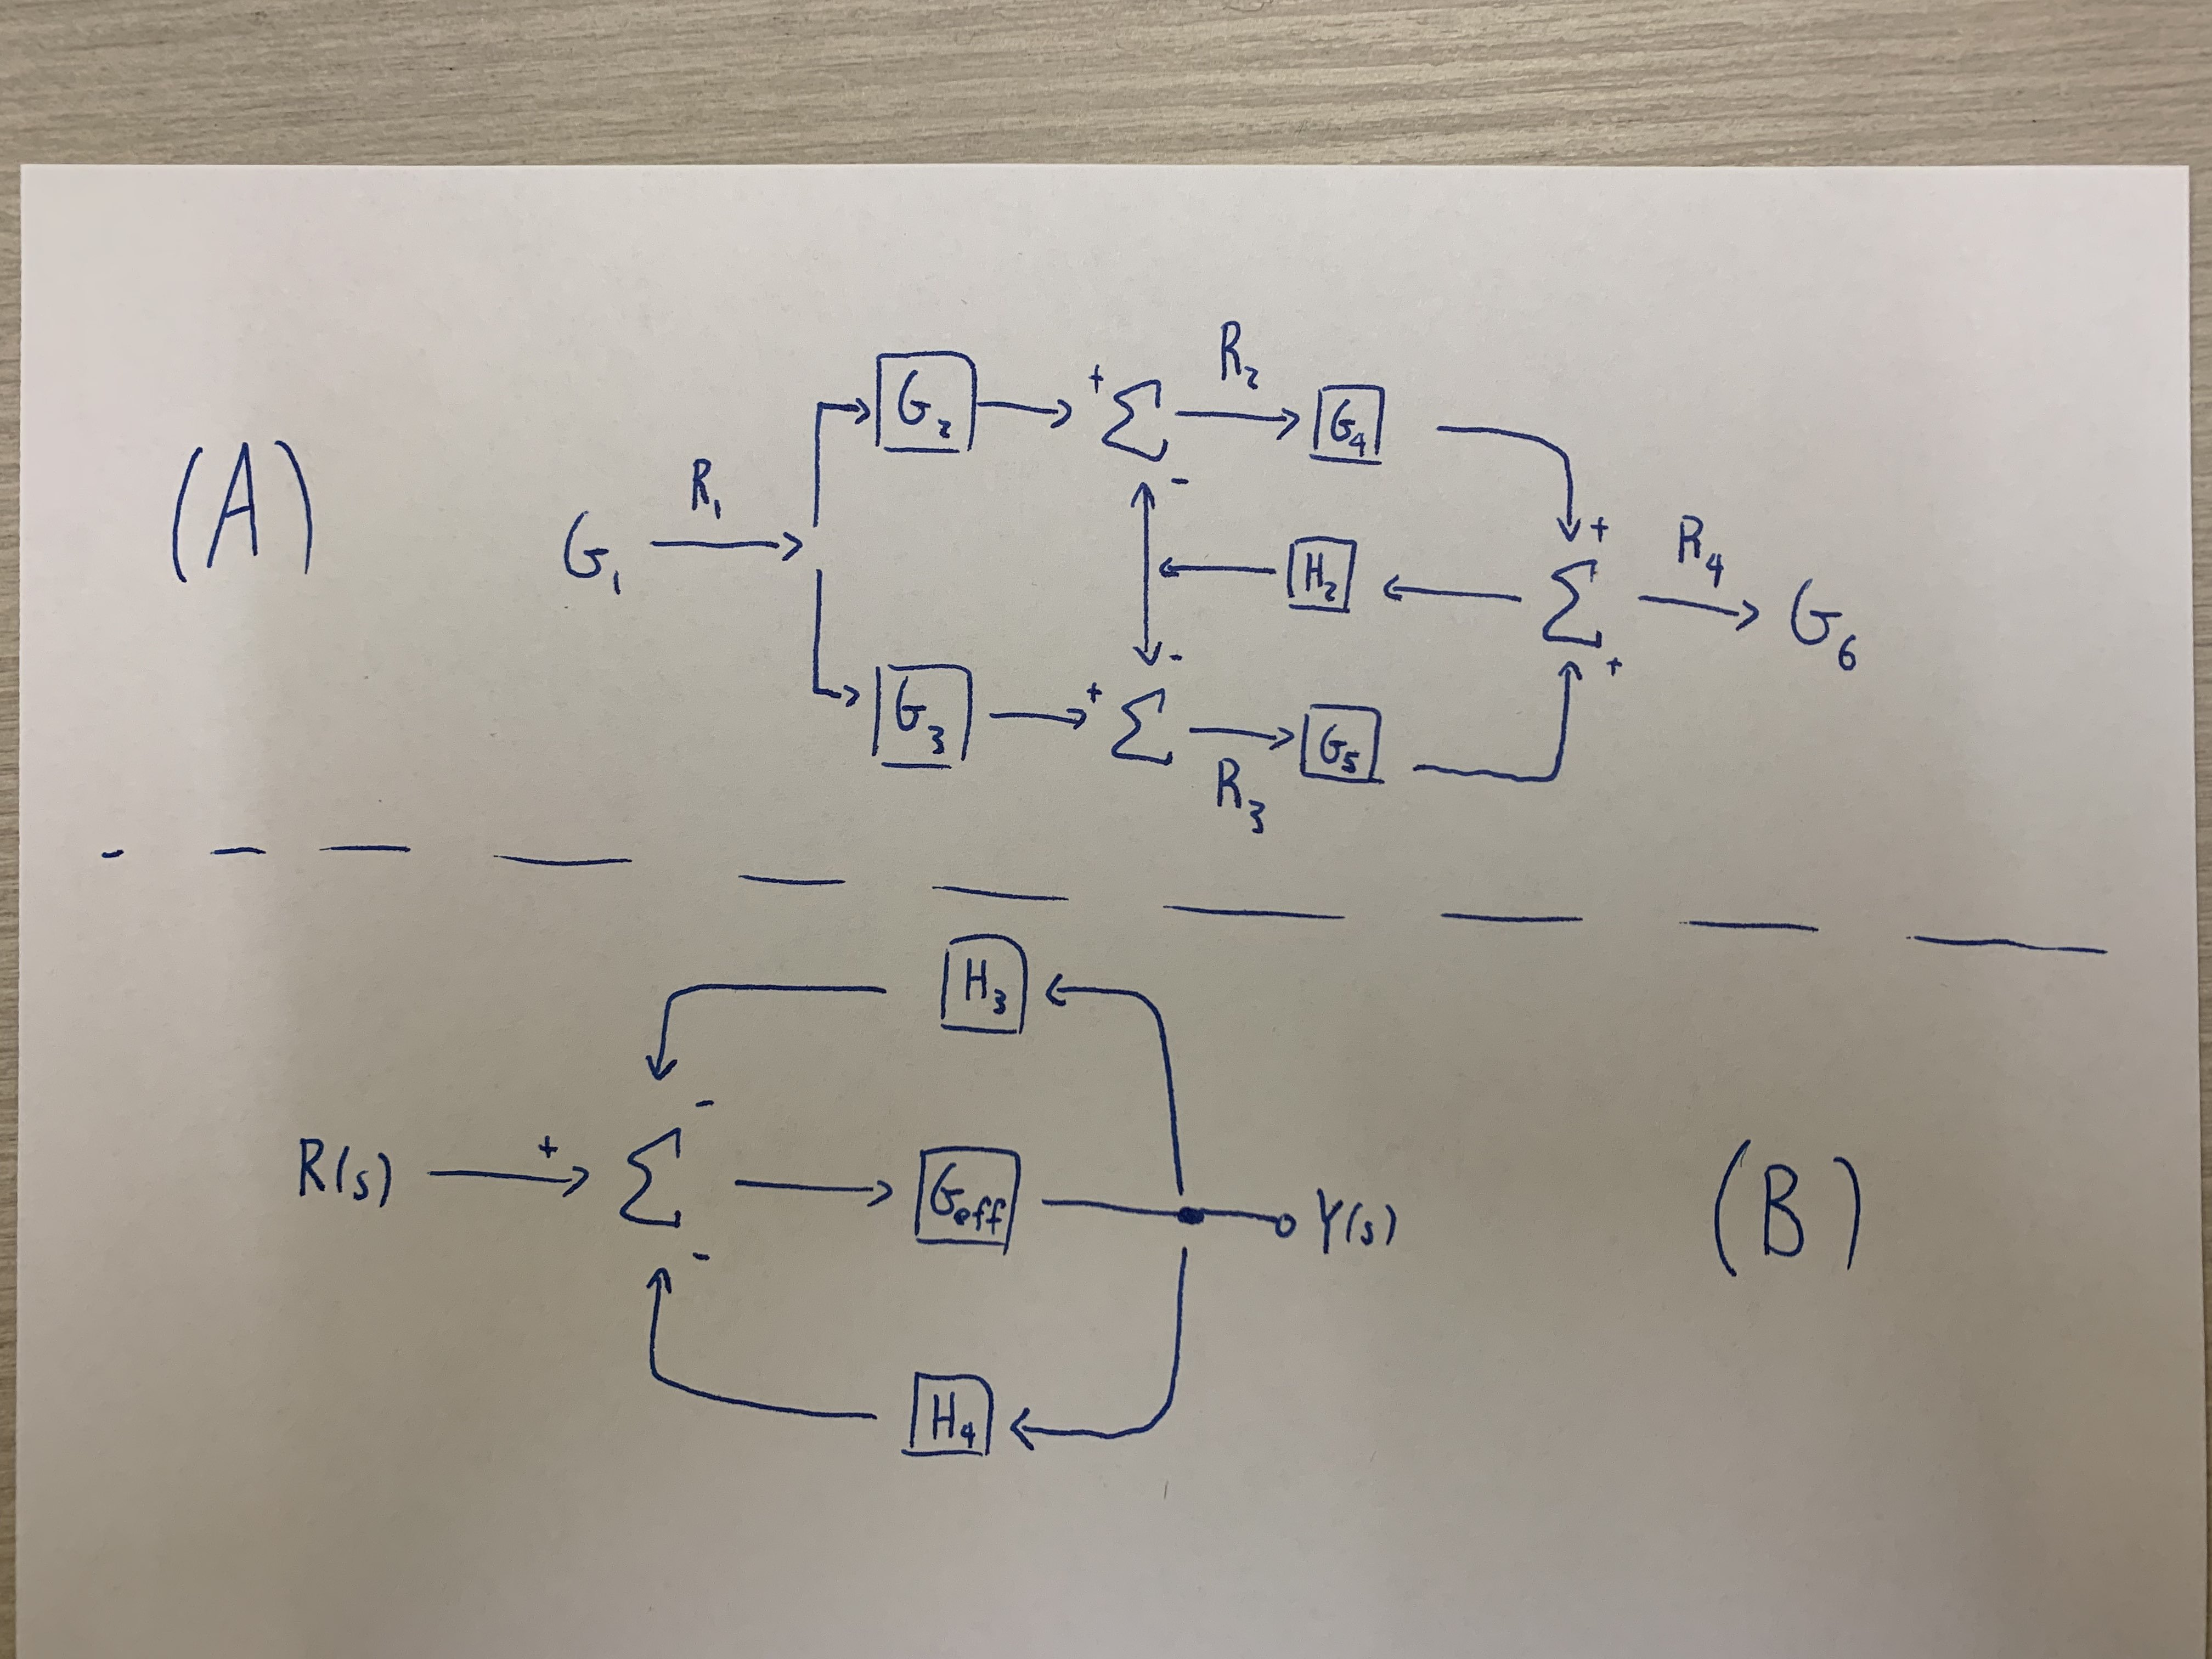
\includegraphics[width=\linewidth]{pset1_q6.jpg}
    \end{center}
    Then,
    \begin{align}
        R_2(s) &= R_1(s)G_2 - H_2\left(R_2(s)G_4 + R_3(s)G_5\right), \\ 
        R_3(s) &= R_1(s)G_3 - H_2\left(R_2(s)G_4 + R_3(s)G_5\right).
    \end{align}
    Multiply both sides of the equation on the first side by $G_4,$ and multiply both sides by $G_5$ for the second equation. We get,
    \begin{align}
        R_2(s)G_4 &= R_1(s)G_2G_5 - H_2G_4\left(R_2(s)G_4 + R_3(s)G_5\right), \\ 
        R_3(s)G_5 &= R_1(s)G_3G_5 - H_2G_5\left(R_2(s)G_4 + R_3(s)G_5\right).
    \end{align}
    Adding these up, we obtain 
    \begin{equation}
        R_2(s)G_4 + R_3(s)G_5 = R_1(s)G_2G_5 - H_2G_4\left(R_2(s)G_4 + R_3(s)G_5\right) + R_1(s)G_3G_5 - H_2G_5\left(R_2(s)G_4 + R_3(s)G_5\right).
    \end{equation}
    But $R_4:=R_2(s)G_4 + R_3(s)G_5$ is the output of the third (rightmost) summing point. Making this substitution, we can solve for $R_4.$
    \begin{equation}
        R_4 = R_1G_2G_4 +R_1G_3G_5 - H_2G_4R_4 - H_2G_5R_4 \implies R_4 = \frac{R_1(s)(G_2G_4+G_3G_5)}{1+H_2(G_4+G_5)}.
    \end{equation}
    Therefore, our diagram is now simpler. See part (B) of the above diagram. The effective feedback is $H_3+H_4$ due to linearity and the effective gain is 
    \begin{equation}
        G_{eff} = \frac{G_1G_6(G_2G_4+G_3G_5)}{1+H_2(G_4+G_5)},
    \end{equation}
    so the transfer function is 
    \begin{align}
        \frac{R(s)}{R(s)} &= \frac{G_{eff}}{1+G_{eff}(H_3+H_4)} \\ 
        &= \frac{G_1G_6(G_2G_4+G_3G_5)}{1+H_2(G_4+G_5)} \cdot \left(1 + \frac{G_1G_6(G_2G_4+G_3G_5)(H_3+H_4)}{1+H_2(G_4+G_5)}\right)^{-1} \\ 
        &= \frac{G_1G_6(G_2G_4+G_3G_5)}{1+H_2(G_4+G_5)} \cdot \left(\frac{1 + H_2(G_4+G_5) + G_1G_6(G_2G_4+G_3G_5)(H_3+H_4)}{1+H_2(G_4+G_5)}\right)^{-1} \\ 
        &= \boxed{\frac{G_1G_6(G_2G_4+G_3G_5)}{1+H_2(G_4+G_5)+G_1G_6(G_2G_4+G_3G_5)(H_3+H_4)}}.
    \end{align}
    \item We have,
    \begin{align}
        \frac{Y(s)}{R(s)} &= \frac{K}{s(s+2)}\left(1 + \frac{K}{s(s+2)}\right)^{-1} \\ 
        &= \frac{K}{s(s+2)} \cdot \frac{s(s+2)}{s(s+2)+K} \\ 
        &= \frac{K}{s^2+2s+K}
    \end{align}
    The Laplace transform of a unit step is $\frac{1}{s},$ so we can write $C(s)$ as 
    \begin{align}
        C(s) &= \frac{1}{s(s^2+2s+K)} \\ 
        &= \frac{1}{s} - \frac{s+2}{s^2+2s+K},
    \end{align}
    through partial fraction decomposition. Further making the substitution
    \begin{equation}
        s^2+2s+K = (s+1)^2 + (K-1)
    \end{equation}
    gives 
    \begin{equation}
        \frac{s+1}{(s+1)^2 + K - 1} + \frac{1}{\sqrt{K-1}} \cdot \frac{\sqrt{K-1}}{(s+1)^2 + K -1},
    \end{equation}
    allowing us to decompose $C(s)$ into three terms we can easily take the inverse Laplace transform of. We have,
    \begin{align}
        c(t) &= \mathcal{L}^{-1}\left\{C(s)\right\} \\ 
        &= \mathcal{L}^{-1}\left\{\frac{1}{s} - \frac{s+1}{(s+1)^2 + K - 1} - \frac{1}{\sqrt{K-1}} \cdot \frac{\sqrt{K-1}}{(s+1)^2 + K -1}\right\} \\ 
        &= 1 + e^{-t}\cos\left(\sqrt{K-1}t\right) + e^{-t}\frac{1}{\sqrt{K-1}}\sin\left(\sqrt{K-1}t\right).
    \end{align}
    Recall that $u(t) = 1$ for $t > 0.$ Note this is only valid for $K>0,$ which is an assumption we will need to check at the end. We can further simplify things by making the substitution $\omega_n = \sqrt{K-1}$ and the identity 
    \begin{equation}
        A\sin(x)+B\cos(x) = \sqrt{A^2+B^2}\sin\left(x + \arctan(B/A)\right)
    \end{equation}
    to obtain 
    \begin{equation}
        c(t) = 1 + \sqrt{1+\frac{1}{\omega_n^2}}e^{-t}\sin\left(\omega_n t + \arctan(\omega_n)\right)
    \end{equation}
    The peak time can be determined by finding when $c(t)$ is extremized. Taking the time derivative and setting it to zero,
    \begin{align}
        &0 = \frac{d}{dt}\left(1 + \sqrt{1+\frac{1}{\omega_n^2}}e^{-t}\sin\left(\omega_n t + \arctan(\omega_n)\right)\right) \\ 
        \implies & 0 = -e^{-t}\sin(\omega_n t + \arctan(\omega_n)) + \omega_n e^{-t}\cos(\omega_n t + \arctan(\omega_n)) \\ 
        \implies &\tan(\omega_n t + \arctan(\omega_n)) = \omega_n \\ 
        \implies & \omega_n t + \arctan(\omega_n) = \arctan(\omega_n) + k\pi,\\ 
        \implies & \omega_n t = k\pi,
    \end{align}
    where $k$ is a non-negative integer. There are potentially an infinite number of extreme points, but we know that the one that corresponds to the first positive $t_p$ corresponds to the peak time since the envelope function $e^{-t}$ is strictly decreasing, so we chose $k=1$ to obtain $t_p = \frac{\pi}{\omega_n}.$
    
    The maximum overshoot is,
    \begin{align}
        M &= \left|\frac{c(t_p) - c(\infty)}{c(\infty)}\right| \\ 
        &= |c(t_p) - 1| \\ 
        &= \sqrt{1+\frac{1}{\omega_n^2}}e^{-t_p}|\sin\left(\omega_n t_p + \arctan(\omega_n)\right)| \\ 
        &= \sqrt{1+\frac{1}{\omega_n^2}} e^{-\pi/\omega_n}|\sin(\pi + \arctan(\omega_n))| \\ 
        &= \sqrt{\frac{\omega_n^2+1}{\omega_n^2}} e^{-\pi/\omega_n} \frac{\omega_n}{\sqrt{\omega_n^2+1}} \\ 
        &= e^{-\pi/\omega_n}.
    \end{align}
    To simplify, the identity 
    \begin{equation}
        \sin(\arctan(x)) = \frac{x}{\sqrt{x^2+1}}
    \end{equation}
    was used. We want this to have a value of $10\%,$ so 
    \begin{equation}
        \omega_n = \frac{-\pi}{\ln(0.1)},
    \end{equation}
    and so 
    \begin{equation}
        K = \omega_n^2 +1 = 1 + \pi^2 \frac{1}{\log(0.1)^2},
    \end{equation}
    or 
    \begin{equation}
        \boxed{1 < K < 2.862.}
    \end{equation}
    Note that decreasing $K$ will decrease $\omega_n$ which will increase $M.$ The smallest $K$ can be is $1,$ because of our earlier assumption. Past that, our system turns from an under-damped system to a critically-damped or over-damped system, where the overshoot doesn't exist anymore (and therefore doesn't make sense to talk about it). 
    \item \begin{enumerate}[label=(\alph*)]
        \item First, we can determine the closed loop gain to be 
        \begin{align}
            \frac{Y(s)}{R(s)} &= \frac{G}{1+G} \\ 
            &= \frac{K}{s(s+2)} \cdot \frac{s(s+2)}{K+s(s+2)} \\ 
            &= \frac{K}{s^2+2s+K}, 
        \end{align}
        which is the same as in the previous problem. We have already shown that 
        \begin{equation}
            t_p = \frac{\pi}{\sqrt{K-1}},\quad\quad\quad\quad 1 < K < 1 + \frac{\pi^2}{\ln(M_p)}.
        \end{equation}
        If $t_p=1\text{ sec},$ then 
        \begin{equation}
            K = \left(\frac{\pi}{t_p}\right)^2 + 1 = 1 + \pi^2 \approx 10.87.
        \end{equation}
        The second condition gives 
        \begin{equation}
            K < 1 + \frac{\pi^2}{\ln(0.05)^2} \approx 2.0997,
        \end{equation}
        so the conditions cannot be simultaneously satisfied.
        \item The transfer function has poles at 
        \begin{equation}
            s = -1 \pm \sqrt{1-K}.
        \end{equation}
        There are two cases. If $K \le 1,$ then $s \in (-\infty, 1].$ If $K > 1,$ we have $s \in \{-1\} \times \mathbb{R} \subseteq \mathbb{C}.$ This is plotted in the blue lines.

        We have two conditions we wish to satisfy. To determine general formulas for the roots that satisfy these conditions, we first need to write the transfer function in the most general form,
        \begin{equation}
            H(s) = \frac{\omega_n^2}{s^2 + 2\zeta\omega_n s + \omega_n^2}
        \end{equation}
        which has an overshoot of 
        \begin{equation}
            M_p = \exp\left(-\frac{\pi\zeta}{\sqrt{1-\zeta^2}}\right) < 5\%.
        \end{equation}
        Note that 
        \begin{align}
            \left|\frac{\text{Im}(s)}{\text{Re}(s)}\right| = \frac{\omega_d}{\zeta\omega_n} = \pm\frac{\sqrt{1-\zeta^2}}{\zeta},
        \end{align}
        so the $M_p<5\%$ condition gives 
        \begin{equation}
            \left|\frac{\text{Re}(s)}{\text{Im}(s)}\right| < -\frac{\ln(0.05)}{\pi} \implies |\text{Im}(s)| < -1.049\text{Re}(s),
        \end{equation}
        which gives the region bounded by the two red lines. Finally, we have the condition that $t_p \le 1\text{ s}.$ The peak time is given by 
        \begin{equation}
            t_p \le \frac{\pi}{|\text{Im}(s)|} \implies |\text{Ims}(s)| \ge \pi,
        \end{equation}
        where the boundary is plotted in green.
        \begin{center}
            \begin{tikzpicture}
            \begin{axis}[
            legend pos=outer north east,
            title=s-plane for Satisfication of Conditions,
            axis lines = middle,
            xlabel = $\mathbb{R}$,
            ylabel = $\mathbb{C}$,
            variable = t,
            trig format plots = rad,
            ymin=-5,
            ymax=5,
            xmax=2,
            ]
            \addplot [
                domain=-4:1,
                samples=70,
                color=blue,
                ultra thick,
                forget plot
                ]
                {0};
            \addplot [color=blue, ultra thick]
                table[row sep=crcr]{%
            -1   -5\\
            -1   5\\
            };
            \addlegendentry{Poles of $H(s)$}
            \addplot [
                domain=-4:0,
                samples=70,
                color=red,
                ultra thick,
                forget plot
                ]
                {-1.05*x};
            \addplot [
                domain=-4:0,
                samples=70,
                color=red,
                ultra thick
                ]
                {1.05*x};
            \addlegendentry{$M_p < 5\%$ condition}
            \addplot [
                domain=-4:0,
                samples=70,
                color=green,
                ultra thick,
                forget plot
                ]
                {pi};
            \addplot [
                domain=-4:0,
                samples=70,
                color=green,
                ultra thick
                ]
                {-pi};
            \addlegendentry{$t_p < 1s$ condition}
            \end{axis}
            \end{tikzpicture}
        \end{center}
        The region in which the conditions are satisfied are between the red and green curves, which do not intersect the blue curves, so the conditions cannot be satisfied.
        \vspace{2mm}

        Let us explore some possible values of $K.$ If $K \gg 1,$ the roots start at $\text{Re}(s)=-1$ and have very high imaginary values (both signs). As $K$ decreases, these roots come together and collide at $s=-1.$ Then further decreasing $K$ will cause the roots to split apart again, but this time on the real axis, but it will not be symmetric.
        \vspace{2mm}

        Suppose we wish to relax either of our conditions such that we can satisfy it. We deal with two cases:
        \begin{itemize}
            \item What is the maximum accepted value of $t_p$ such that we have a solution? The intersection of the blue and red curves is given by 
            \begin{equation}
                \pm 1.05 \text{Im}(s) = -1 \implies \text{Im}(s) = \pm 0.95 
            \end{equation}
            so we require 
            \begin{equation}
                t_p \le \frac{\pi}{0.95} \approx 3.3\text{ s}.
            \end{equation}
            \item What is the maximum overshoot $M_p$ such that conditions can be met? We want to shift the red curve such that it intersects the blue and green curve at $(\text{Re}(s),\text{Im}(s)) = (-1,\pi).$ We want 
            \begin{equation}
            |\text{Im}(s)| = \frac{\pi}{\ln(M_{p,max})}\text{Re}(s) \implies M_{p,max} = e^{-1} \approx 37\%.
            \end{equation}
        \end{itemize}
    \end{enumerate}
    \item One of the zeros is very close to one of the poles, so we can cancel them out, 
    \begin{align}
        H(s) &\approx \frac{(s/2+1)(s/0.1+1)}{[(s/4)^2+(s/4)+1](s/0.02+1)}.
    \end{align}
    We now look at the dominant behavior: Out of the roots and poles $s=-2,-0.1,-0.02, x=-2 \pm 2j\sqrt{3},$ we have that $s=-0.02$ is closest to the imaginary axis, so this dominates the behavior of the system. Therefore we can approximate the settling time as (pg 51 of chapter 3 - part 3 slides),
    \begin{equation}
        t_s \approx \frac{4.6}{0.02} = 230\text{ s}.
    \end{equation}
    We can verify this using \textit{Mathematica} (although in engineering, will always be mathematician by heart),

    \begin{doublespace}
        \noindent\(\pmb{H[\text{s$\_$}]\text{:=}((s/10){}^{\wedge}2+0.1(s/10)+1)(s/2+1)(s/0.1+1)/(((s/4){}^{\wedge}2+(s/4)+1)((s/10){}^{\wedge}2+0.09(s/10)+1)(s/0.02+1));}\\
        \pmb{H[s]\text{//}\text{DisplayForm}}\)
        \end{doublespace}
        
        \begin{doublespace}
        \noindent\(\frac{\left(1+\frac{s}{2}\right) (1+10. s) \left(1+0.01 s+\frac{s^2}{100}\right)}{(1+50. s) \left(1+0.009 s+\frac{s^2}{100}\right) \left(1+\frac{s}{4}+\frac{s^2}{16}\right)}\)
        \end{doublespace}
        
        \begin{doublespace}
        \noindent\(\pmb{y[\text{t$\_$}]\text{:=}\text{InverseLaplaceTransform}[1/s*H[s],s,t]}\)
        \end{doublespace}
        
        \begin{doublespace}
        \noindent\(\pmb{\text{Plot}[y[t],\{t,0,230\}]}\)
        \end{doublespace}
        
        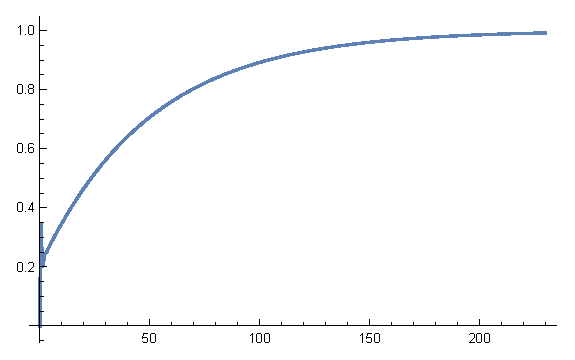
\includegraphics{pset1_gr1.eps}
        
        \begin{doublespace}
        \noindent\(\pmb{\text{FindRoot}[y[t]\text{==}0.99,\{t,230\}]}\)
        \end{doublespace}
        
        \begin{doublespace}
        \noindent\(\{t\to 218.847\, -\text{3.5605271890862875$\grave{ }$*${}^{\wedge}$-61} i\}\)
        \end{doublespace}
        
        So we get around $220\text{ s},$ which is very close to our estimate! Because this is approximated by a first order system, there is no overshoot.
\item \begin{enumerate}[label=(\alph*)]
    \item We have critical damping. If we have repeated roots, then we can factor
    \begin{equation}
        H(s) = \frac{\omega_n^2}{(s+\omega_n)^2},
    \end{equation}
    i.e. $\zeta = 1.$ To impulse response is 
    \begin{equation}
        y(t) = \mathcal{L}^{-1}\{H(s)\} = \omega_n^2 te^{-\omega_n t}
    \end{equation}
    and the step response is 
    \begin{align}
        y(t) &= \mathcal{L}^{-1}\{\frac{1}{s}H(s)\} \\ 
        &= \mathcal{L}^{-1}\left\{\frac{1}{s} - \frac{1}{s+\omega_n} - \frac{\omega_n}{(s+\omega_n)^2}\right\} \\ 
        &= 1 - e^{-\omega_n t} - \omega_n te^{-\omega_n t}.
    \end{align}
    \item We have an over-damped system. If the roots are real, then the discriminant is positive,
    \begin{equation}
        4\zeta^2\omega_n^2-4\omega_n^2 > 0 \implies 1-\zeta^2 < 0.
    \end{equation}
    Let us set $\gamma^2 = \omega_n^2(\zeta^2-1).$ Then by partial fraction decomposition,
    \begin{align}
        H(s) &= \frac{\omega_n^2}{(s+\zeta \omega_n)^2 - \gamma^2} \\ 
        &= \frac{\omega_n^2}{2\gamma(s -\gamma  + \omega_n \zeta)} + \frac{\omega_n^2}{2\gamma(s +\gamma  + \omega_n \zeta)}.
    \end{align}
    The inverse Laplace transform gives the impulse response,
    \begin{align}
        y(t) = \frac{\omega_n^2}{\gamma}e^{-\omega_n\zeta t}\sinh(\gamma t) = \frac{\omega_n}{\sqrt{\zeta^2-1}}e^{-\omega_n\zeta t}\sinh(\gamma t).
    \end{align}
    The step response is given by 
    \begin{align}
        y(t) &= \mathcal{L}^{-1}\left\{\frac{1}{s}H(s)\right\} \\ 
        &= \mathcal{L}^{-1}\left\{
            -\frac{\omega_n^2}{s(\gamma^2-\omega_n^2\zeta^2)} + \frac{\omega_n^2}{2\gamma(\gamma - \omega_n\zeta)(s -\gamma + \omega_n \zeta)} + \frac{\omega_n^2}{2\gamma(\gamma + \omega_n\zeta)(s +\gamma + \omega_n \zeta)}
        \right\} \\ 
        &= \frac{\omega_n^2}{\omega_n^2\zeta^2-\gamma^2} + \frac{\omega_n^2}{2\gamma^2-2\gamma \omega_n \zeta}e^{-\omega_n \zeta t}e^{\gamma t} + \frac{\omega_n^2}{2\gamma^2 + 2\gamma \omega_n \zeta}e^{-\omega_n \zeta t}e^{-\gamma t} \\ 
        &= \frac{\omega_n^2}{\omega_n^2\zeta^2-\gamma^2} + \frac{\omega_n^2}{2\gamma}e^{-\omega_n \zeta t}\left(\frac{e^{\gamma t}}{\gamma- \omega_n \zeta} + \frac{e^{-\gamma t}}{\gamma+ \omega_n \zeta}\right) \\ 
        &= \frac{\omega_n^2}{\omega_n^2\zeta^2-\gamma^2} + \frac{\omega_n^2}{2\gamma}e^{-\omega_n \zeta t}\left(\frac{e^{\gamma t}(\gamma+\omega_n\zeta) + e^{-\gamma t}(\gamma - \omega_n\zeta)}{\gamma^2- \omega_n^2 \zeta^2}\right) \\ 
        &= \frac{\omega_n^2}{\omega_n^2\zeta^2-\gamma^2} + \frac{\omega_n^2}{2\gamma}e^{-\omega_n \zeta t}\left(\frac{(\cosh \gamma t + \sinh \gamma t)(\gamma+\omega_n\zeta) + (\cosh \gamma t- \sinh \gamma t)(\gamma - \omega_n\zeta)}{\gamma^2- \omega_n^2 \zeta^2}\right) \\ 
        &= \frac{\omega_n^2}{\omega_n^2\zeta^2-\gamma^2} + \frac{\omega_n^2}{2\gamma}e^{-\omega_n \zeta t}\left(\frac{2\gamma \cosh \gamma t + 2 \omega_n \zeta \sinh \gamma t}{\gamma^2- \omega_n^2 \zeta^2}\right) \\ 
        &= \frac{\omega_n^2}{\omega_n^2\zeta^2 - \gamma^2}\left(1 -e^{-\omega_n\zeta t}\left[ \cosh(\gamma t) + \frac{\omega_n\zeta}{\gamma}\sinh \gamma t\right] \right) \\ 
        &= 1 - e^{-\omega_n\zeta t}\left(\cosh(\gamma t) + \frac{\zeta}{\sqrt{\zeta^2-1}}\sinh \gamma t\right).
    \end{align}
    \item To avoid a lot of the brute force, we rely on symmetries. Note that we can perform the exact same steps as before, but now $\gamma$ is imaginary. Therefore, instead of writing
    \begin{equation}
        e^{\pm \gamma t} = \cosh(\gamma t) \pm \sinh(\gamma t),
    \end{equation}
    for $\gamma\in\mathbb{R},$ we can write 
    \begin{equation}
        e^{\pm j|\gamma| t} = \cos(|\gamma| t) \pm j \sin(|\gamma| t),
    \end{equation}
    which gives us 
    \begin{equation}
        1 - e^{\omega_n|\zeta| t}\left(\cos(|\gamma|t) + \frac{\zeta}{\sqrt{1-\zeta^2}}\sin(|\gamma|t)\right),
    \end{equation}
    where we used the fact that $\sqrt{\zeta^2-1} = j\sqrt{1-\zeta^2},$ to ensure that the step response is real. Similarly, for the impulse response, we have
    \begin{align}
        y(t) &= \frac{\omega_n}{j\sqrt{1-\zeta^2}}e^{\omega_n|\zeta| t}\sinh(j |\gamma| t) \\ 
        &= \frac{1}{2}\frac{\omega_n}{j\sqrt{1-\zeta^2}}e^{\omega_n|\zeta| t}(e^{j|\gamma| t} - e^{-j|\gamma| t}) \\ 
        &= \frac{\omega_n}{\sqrt{1-\zeta^2}}e^{\omega_n|\zeta|t} \sin(|\gamma|t).
    \end{align}
\end{enumerate}
\end{enumerate}

\end{document}